\chapter{Neural Network parameters analysis}
\section{Basic system}
\subsection{First results}

We will see the performance of the Neural Network in approximating the perturbation %
of the basic system. The perturbation is given by \( a \sin(t) \) with \( a = 5 \). %

The default parameters of the Neural Network are as follows:
\begin{itemize}
    \item \textbf{Number of neurons in the hidden layer}: n = 50
    \item \textbf{Learining rate}: \(\gamma\) = 0.075
\end{itemize}

We can plot the mean squared error for each default parameter : 

\begin{figure}[htbp]
    \centering
    \begin{subfigure}{0.49\textwidth}
        \centering
        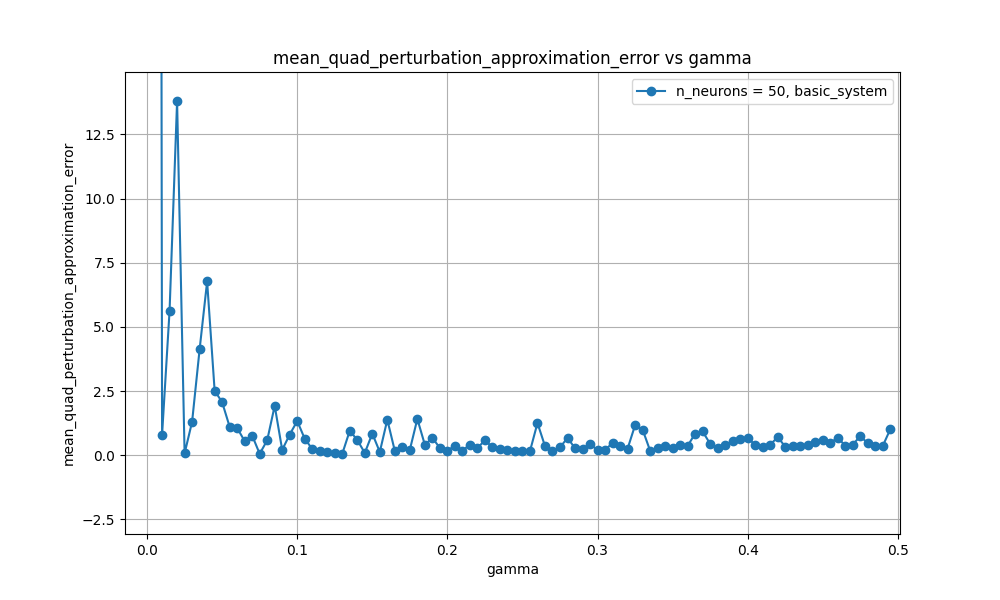
\includegraphics[width=\linewidth]{imgs/section1/plot_nconst50_basicsys.png}
        \caption{MSE, basic system with \(n = 50\)}
        \label{fig:plot_nconst50_basicsys}
    \end{subfigure}
    \hfill
    \begin{subfigure}{0.49\textwidth}
        \centering
        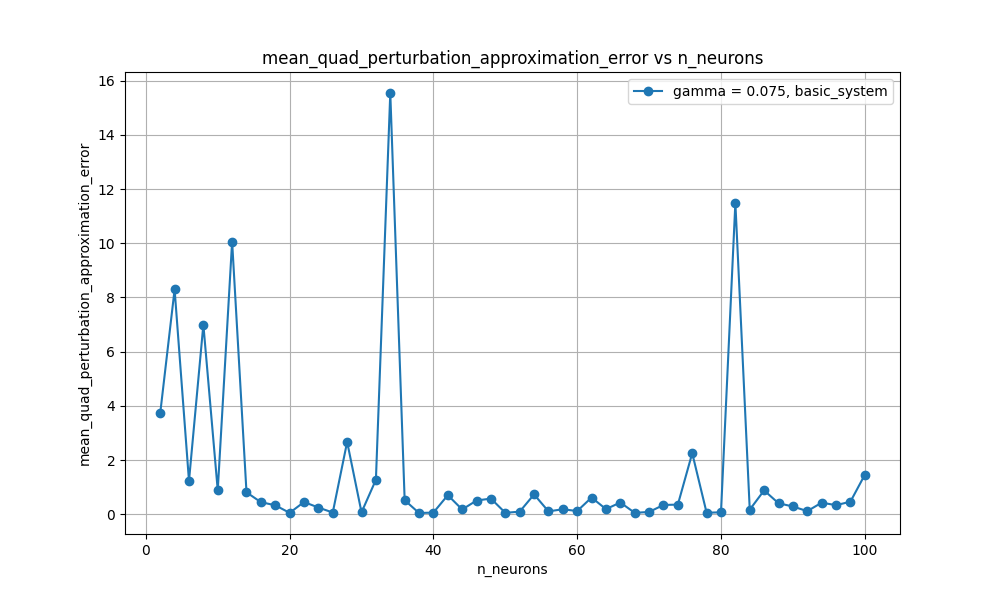
\includegraphics[width=\linewidth]{imgs/section1/plot_gconst0_075_basicsys.png}
        \caption{MSE, basic system with \(\gamma = 0.075\)}
        \label{fig:plot_gammconst075_basicsys}
    \end{subfigure}
    \caption{MSE for the basic system}
    \label{fig:double_plot_basicsys}
\end{figure}

We can see that the mean squared error is decreasing with the number of neurons and the increase %
of the learning rate. On one hand, the error is stabilising on \(0.7 \pm 0.5\) for \(\gamma > 0.1\). %
Although, it would be intersting to see the same metrics with different values of n. To %
assure this statement. On the other hand, it's difficult to see the impact of the %
neurons number with \(\gamma = cst\). Indeed the error seems to be decreasing with %
the number of neurons but the presence of outliers can alert on the overfit issue. %
It also safe to say that we want more than 25 neurons to have a good approximation. %

These plot give some insights on the performance of the approximation regarding certain %
parameters. Unfortunately, we can only see a part of the dataset and not well. %
We can compute the mean, median and standard divation of the curve to get %
quantitative results. We can go further and plot these results for each constant %
parameters. To resume, we chose a type of error (MSE, standard deviation or correlation), %
we also chose the \textit{"varying"} parameter and the dynamic system. Then we can plot %
the mean, median and standard deviation of the error curve of the \textit{"varying"} parameter %
for each \textit{"constant"} parameter. %

First, here is a plot of the mean, median and standard deviation of the MSE curve of %
the figure. \ref{fig:double_plot_basicsys} :

\begin{figure}[htbp]
    \centering
    \begin{subfigure}{0.49\textwidth}
        \centering
        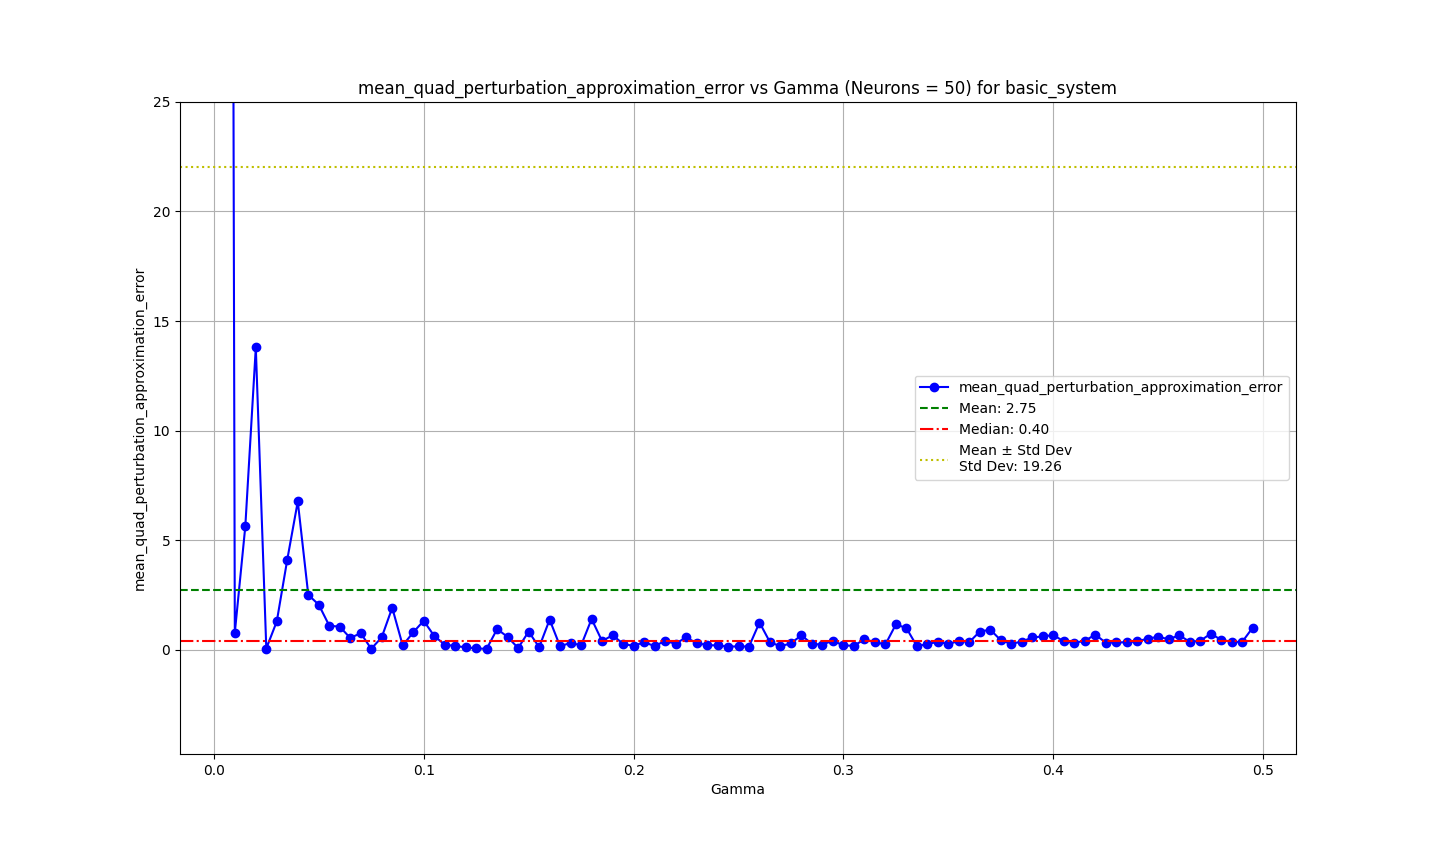
\includegraphics[width=\linewidth]{imgs/section1/error_plot_nconst50_basicsys.png}
        \caption{MSE, basic system with \(n = 50\)}
        \label{fig:error_plot_nconst50_basicsys}
    \end{subfigure}
    \hfill
    \begin{subfigure}{0.49\textwidth}
        \centering
        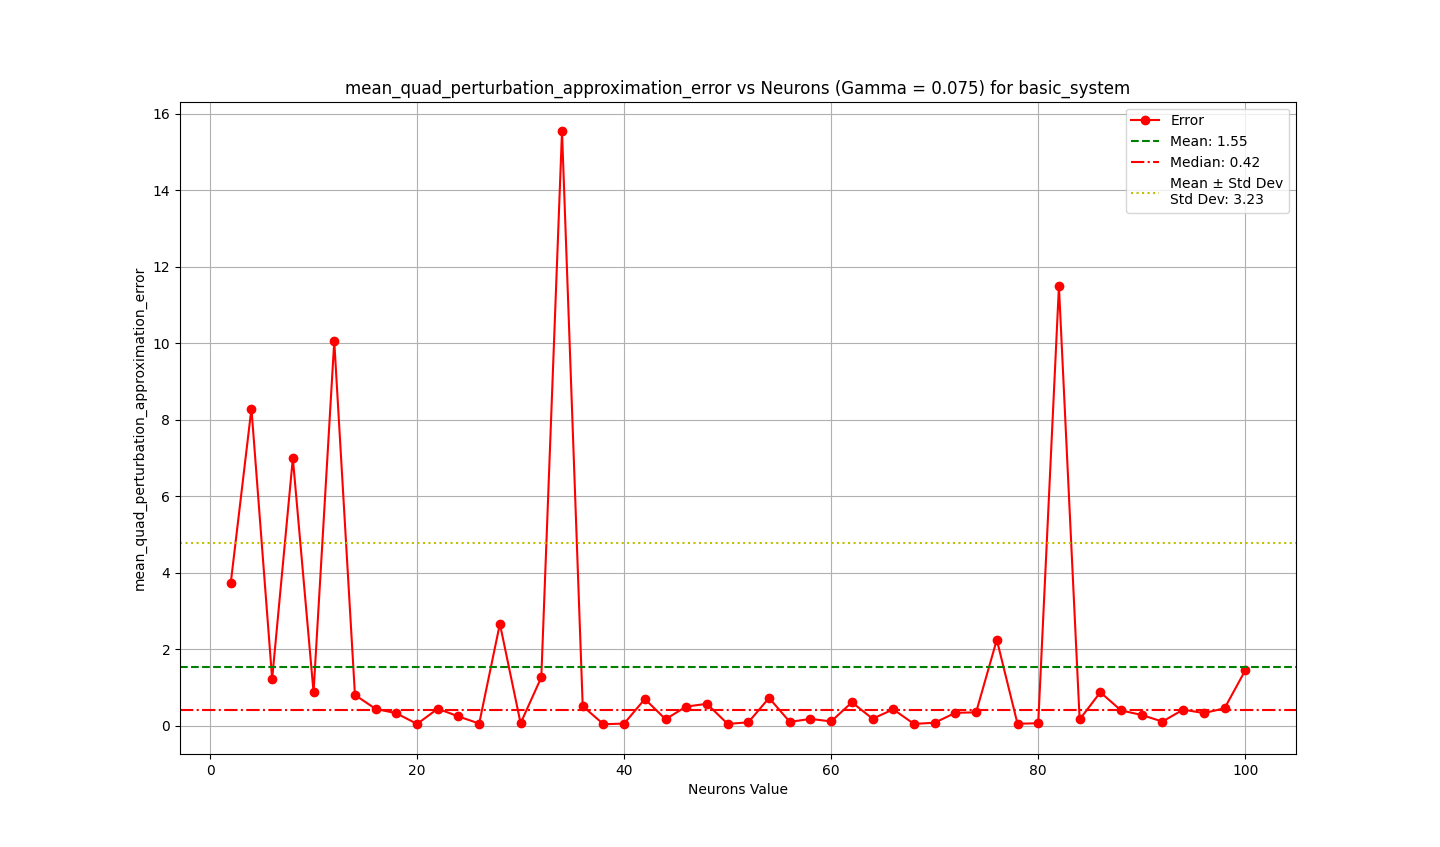
\includegraphics[width=\linewidth]{imgs/section1/error_plot_gconst0_075_basicsys.png}
        \caption{MSE, basic system with \(\gamma = 0.075\)}
        \label{fig:error_plot_gammconst075_basicsys}
    \end{subfigure}
    \caption{MSE for the basic system with its statistics}
    \label{fig:double_error_plot_basicsys}
\end{figure}

Now we can see the impact of the number of neurons and the learning rate on the %
performance of the Neural Network approximation more quantitatively. %

\begin{figure}[htbp]
    \centering
    \begin{subfigure}{0.49\textwidth}
        \centering
        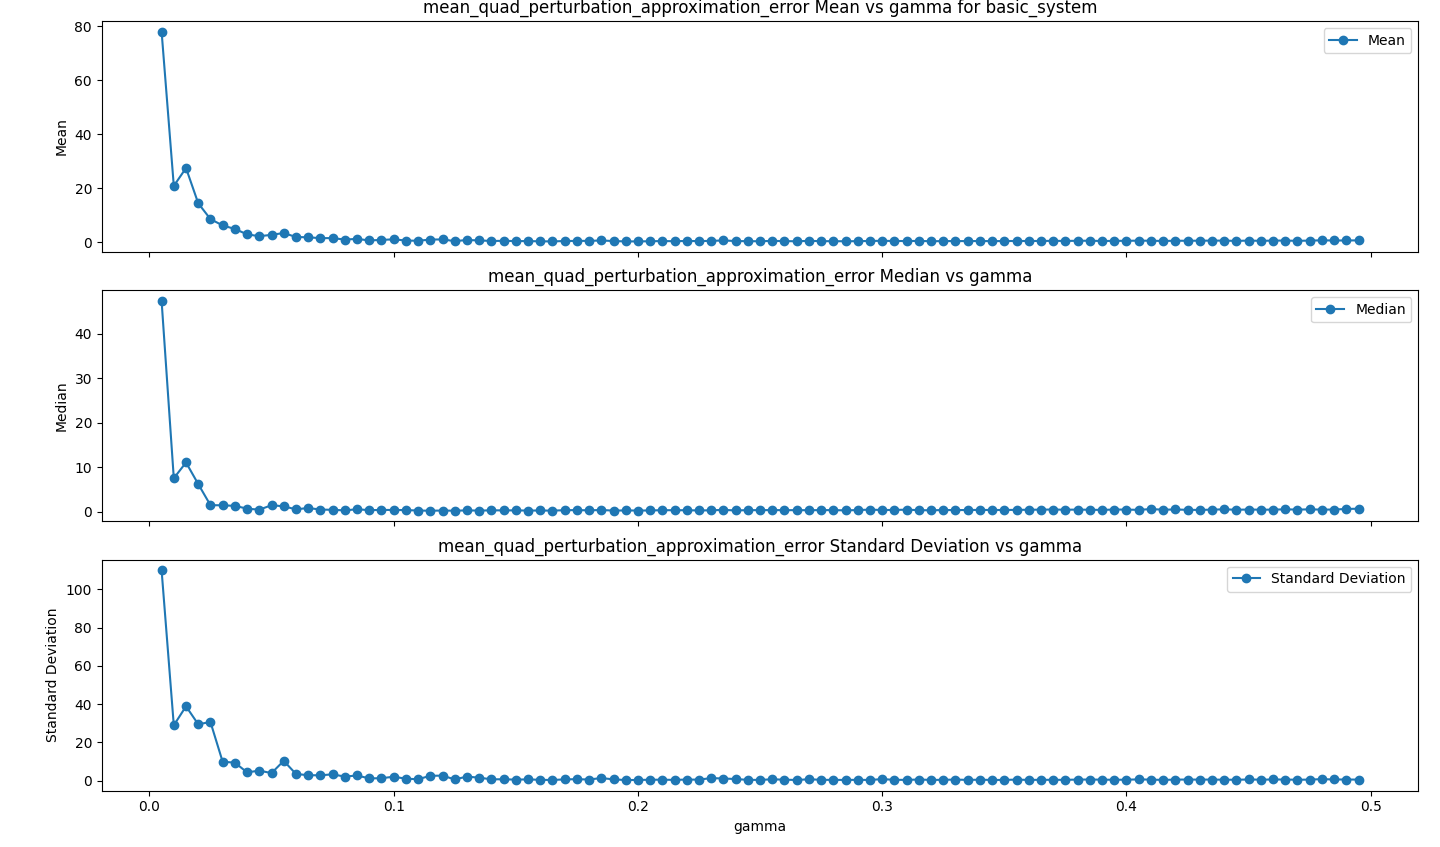
\includegraphics[width=\linewidth]{imgs/section1/MSE_gamma_basic_sys.png}
        \caption{MSE, \(gamma\)}
        \label{fig:MSE_gamma}
    \end{subfigure}
    \hfill
    \begin{subfigure}{0.49\textwidth}
        \centering
        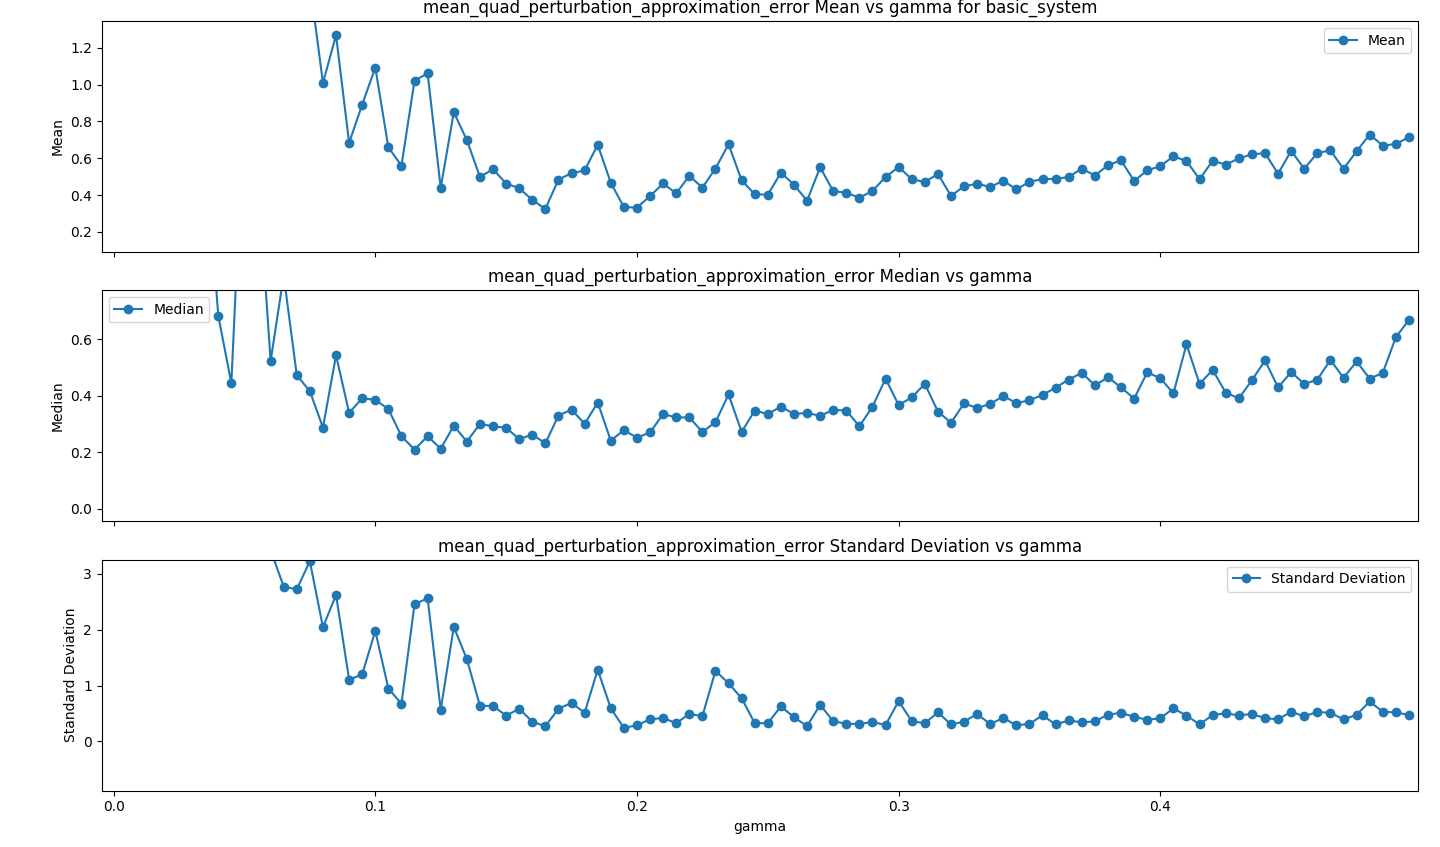
\includegraphics[width=\linewidth]{imgs/section1/MSE_gamma_basic_sys_zoom.png}
        \caption{MSE, \(gamma\) zoomed on y-axis}
        \label{fig:MSE_gamma_zoom}
    \end{subfigure}
    \caption{MSE for all neurons curve for each \(\gamma = cst\)}
    \label{fig:double_plot_basicsysMSEGAMMA}
\end{figure}

\begin{figure}
    \centering
    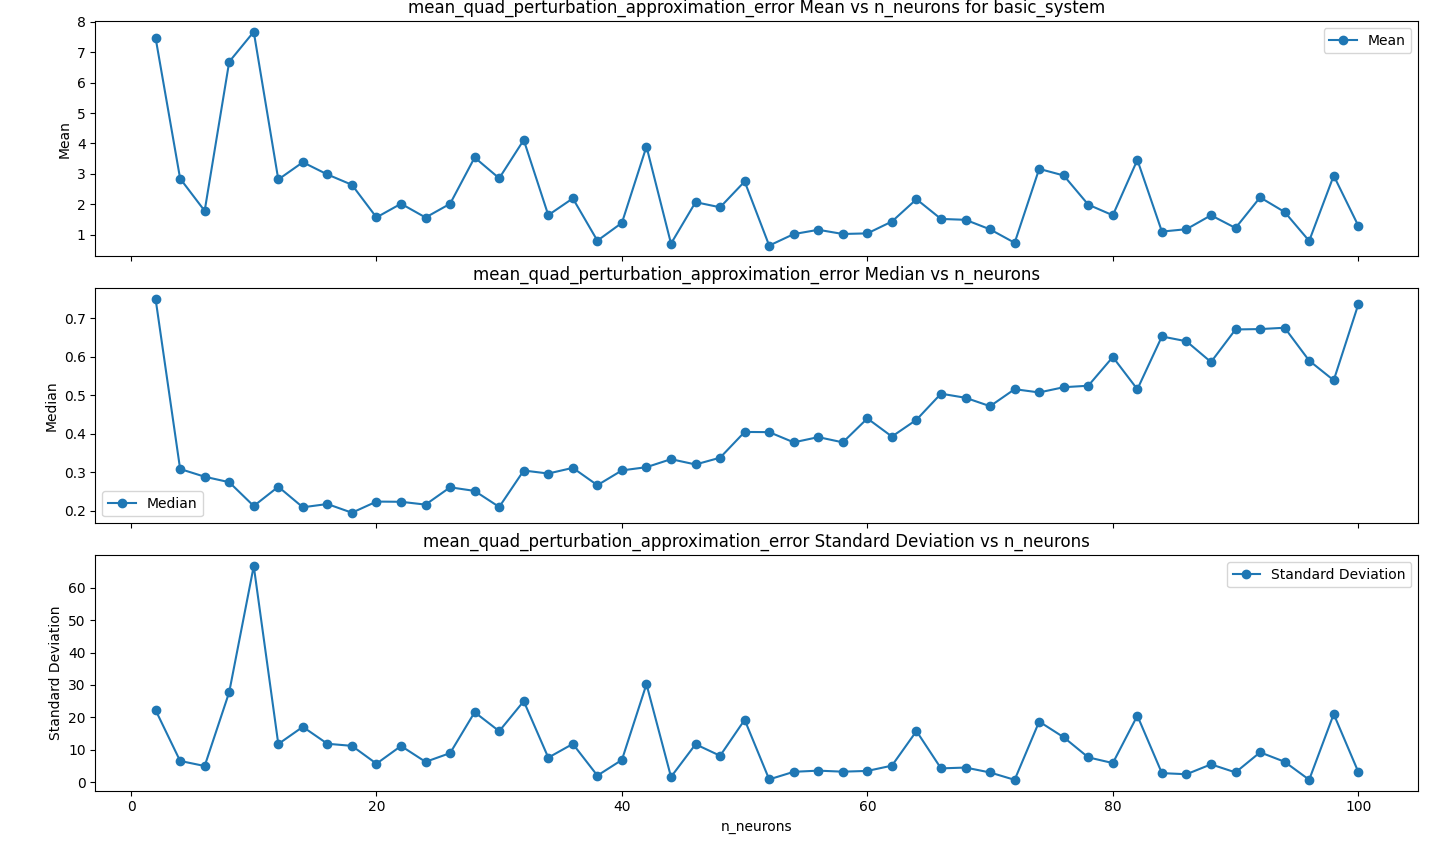
\includegraphics[width=0.8\linewidth]{imgs/section1/MSE_neurons_basic_sys.png}
    \caption{MSE for all \(\gamma\) curve for each \(n\_neurons = cst\)}
    \label{fig:MSE_neurons}
\end{figure}


\subsection{Best tuning region}
We can now see all the plot of median, mean and standard deviation for every error index %
and start to see for which parameters of the Neural Network the approximation is the best. %

\begin{figure}[htbp]
    \centering
    \begin{subfigure}{0.49\textwidth}
        \centering
        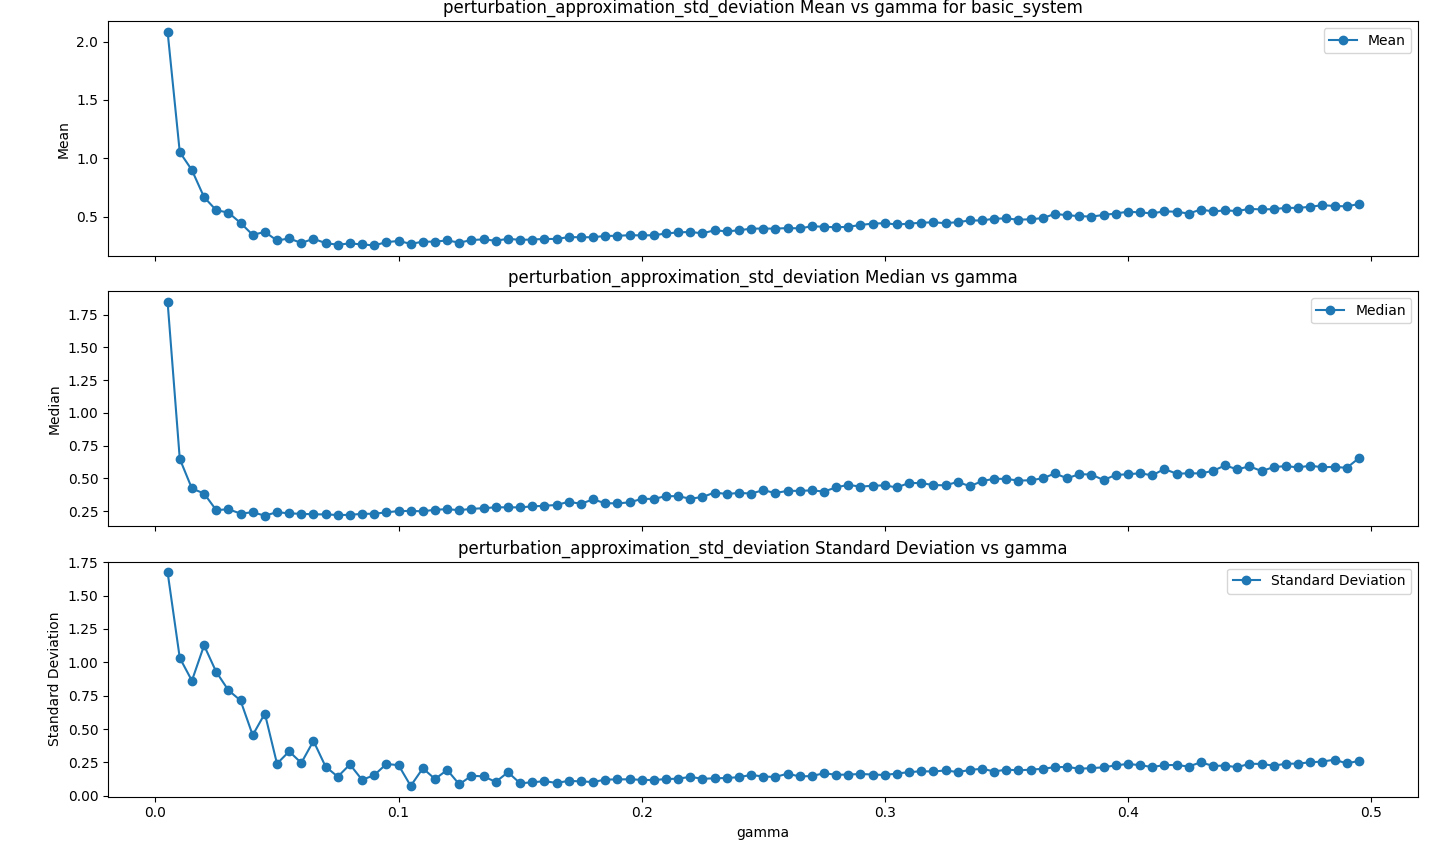
\includegraphics[width=\linewidth]{imgs/section1/stdDev_gamma_basic_sys.png}
        \caption{Standard devation for all neurons curve for each \(\gamma = cst\)}
        \label{fig:stdDev_gamma_basic_sys}
    \end{subfigure}
    \hfill
    \begin{subfigure}{0.49\textwidth}
        \centering
        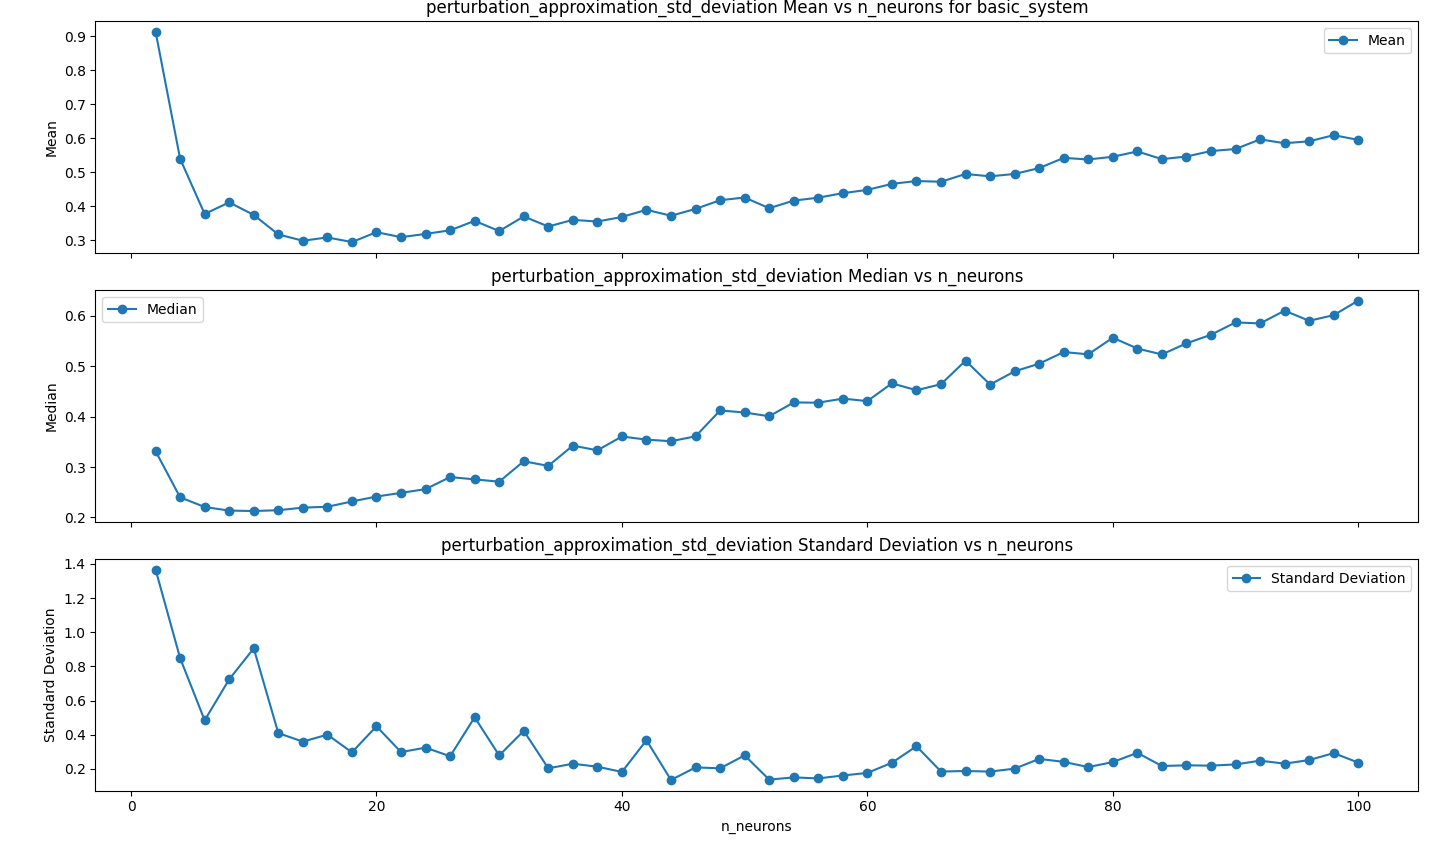
\includegraphics[width=\linewidth]{imgs/section1/stdDev_n_neurones_basic_sys.png}
        \caption{Standard deviation for all \(\gamma\) curve for each \(n\_neurons = cst\)}
        \label{fig:stdDev_n_neurones_basic_sys}
    \end{subfigure}
    \caption{Standard deviations for the basic system}
    \label{fig:Standard_deviations_for_the_basic_system}
\end{figure}

\begin{figure}[htbp]
    \centering
    \begin{subfigure}{0.49\textwidth}
        \centering
        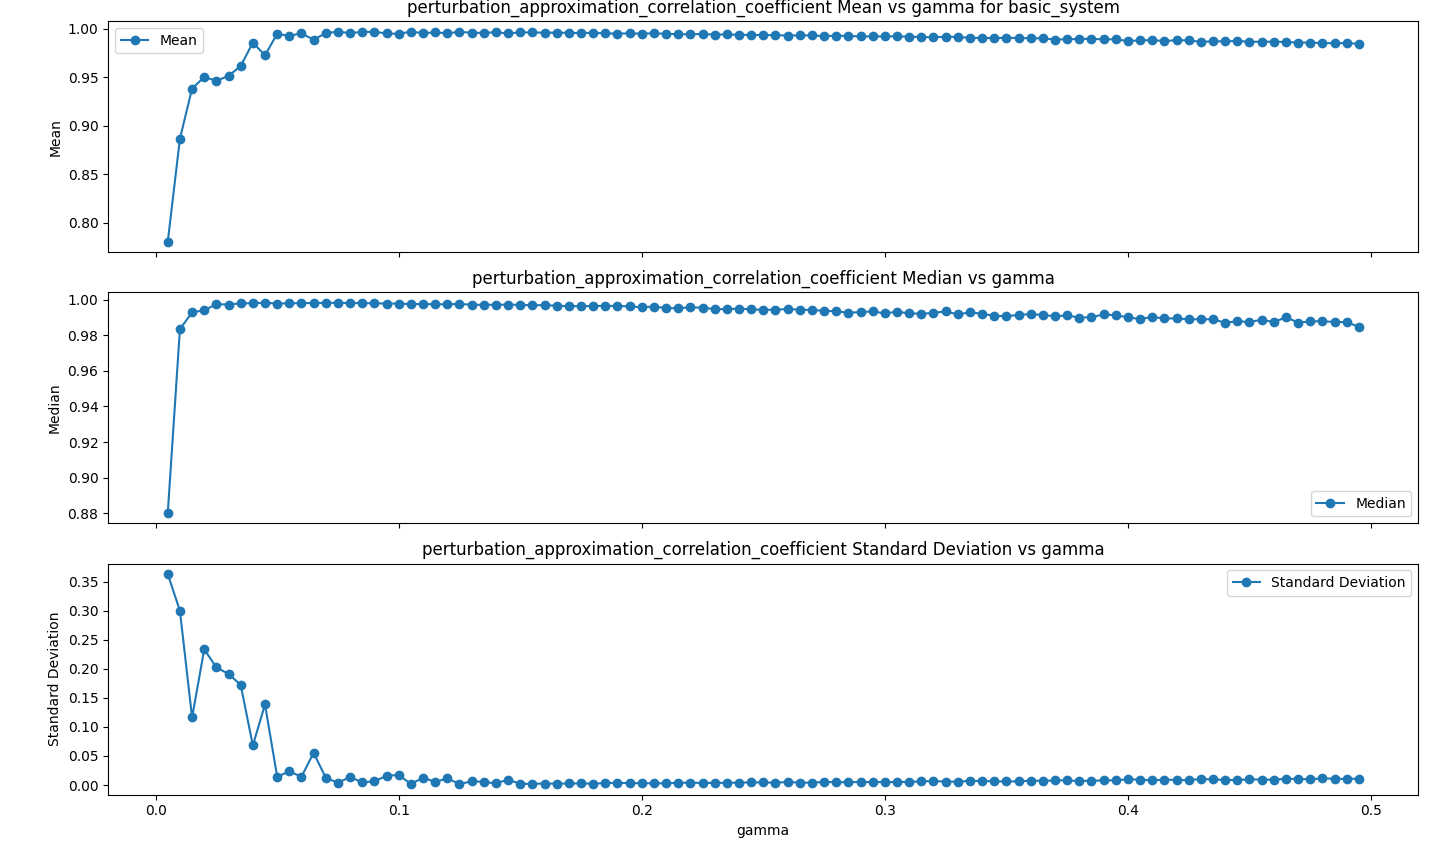
\includegraphics[width=\linewidth]{imgs/section1/corr_gamma_basic_sys.png}
        \caption{Correlation coefficient for all neurons curve for each \(\gamma = cst\)}
        \label{fig:corr_gamma_basic_sys}
    \end{subfigure}
    \hfill
    \begin{subfigure}{0.49\textwidth}
        \centering
        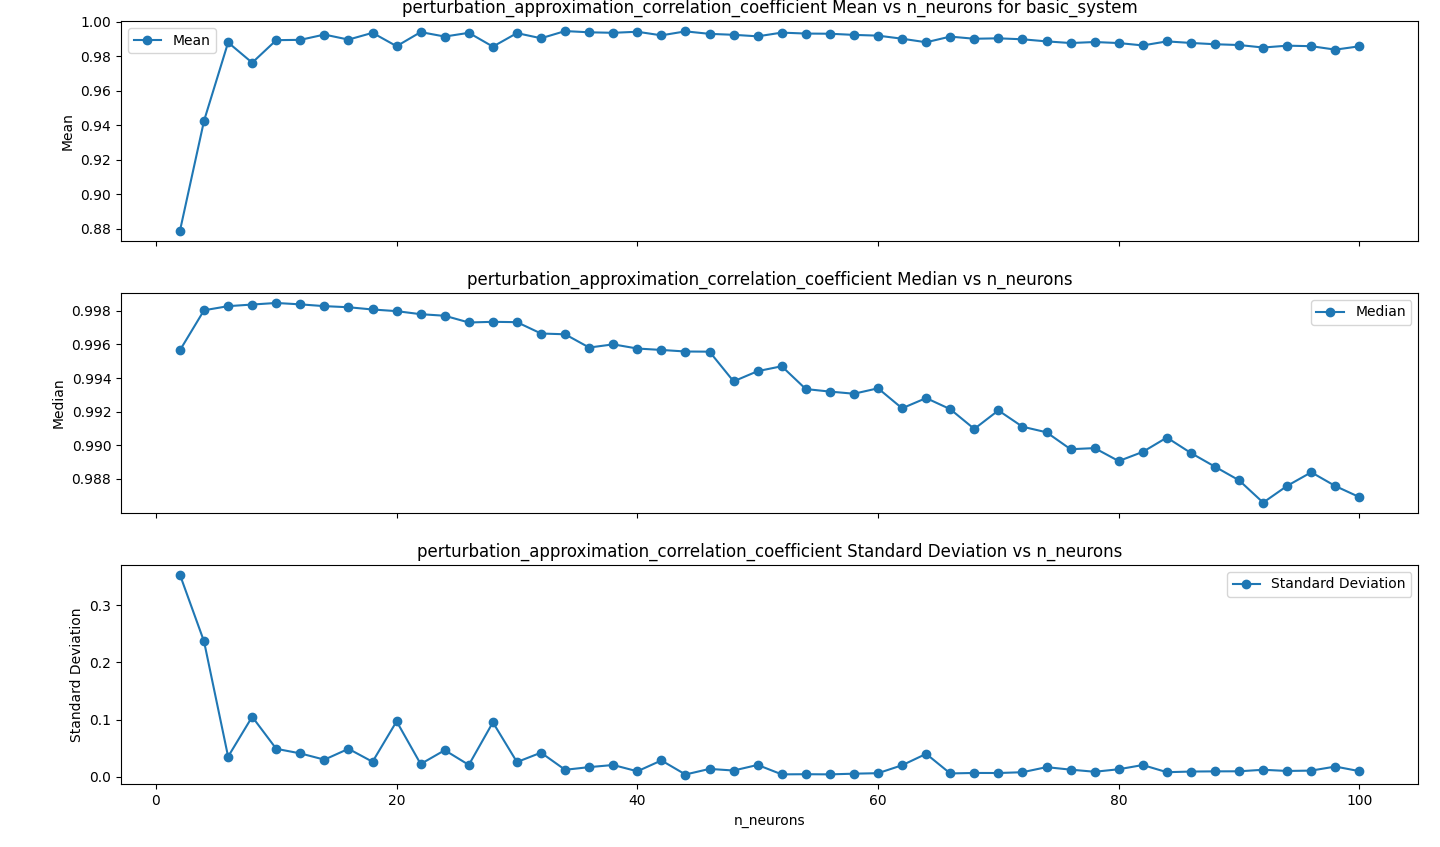
\includegraphics[width=\linewidth]{imgs/section1/corr_n_neurones_basic_sys.png}
        \caption{Correlation coefficient for all \(\gamma\) curve for each \(n\_neurons = cst\)}
        \label{fig:corr_n_neurones_basic_sys}
    \end{subfigure}
    \caption{Correlation coefficient for the basic system}
    \label{fig:Correlation_coefficient_for_the_basic_system}
\end{figure}

We must be careful not to make hasty conclusions. As the standard deviation increase with the %
number of neurons and \(\gamma\), that means that the error is more spread. So can have good % 
results to with high values of \(\gamma\) and \(n\). But  the simulation showed quite %
intersting results.

\subsection{Neural Network questionings}

We can now ask ourselves some questions about the Neural Network : 

\begin{itemize}
    \item What is the Neural Network's contribution to the robustness of the system ?
    \item Could it work with a static gain STWC ?
    \item Can it works in open-loop ? 
    \item The dynamic nature of the weights is really worth it compare to an off-loop Neural Network ?
\end{itemize}

\subsubsection{Open Loop approximation}

By hypothesis, the output of the Neural Network is used in the control law. %
As it is a Lyapunov design, the bondaries of the approximation regarding the %
the real perturbation are assured by the stability of the system that is himself %
assured by the Lyapunov function that used the dynamics of the Neural Network wieghts. %

To resume, there is no reason that the Neural Network approximation is good in open-loop. %

\subsubsection{Static gain approximation}

The proof is based on the fact that the Neural Network works woth an ASTWC. It would be intersting %
to create a new Neural Network that works with a static gain and tune them to unable the control %
to counter the perturbation and see if the Neural Network add some robustness to the system. %

But as we said before, we have to find new dynamic weights definition.

\subsubsection{Neural Network contribution}

It is prooved in Mohammad article that the ouput presents less chattering with the Neural Network. %
We can see that the gains are also smaller du to the anticipation of the perturbation dynamics. %

But, the analysis shows that the approximation's  quality is linked to the stability of the system. %
If the system isn't reaching the sliding surface quickly, the Neural Network will not be able to %
approximate the perturbation. %



\newpage